
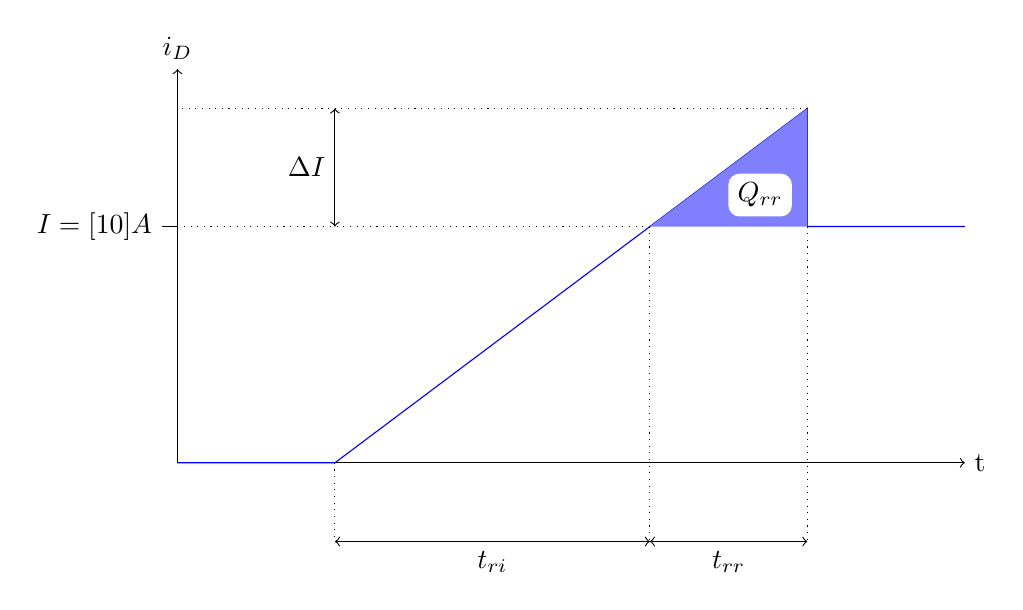
\begin{tikzpicture}%[node distance = 2 cm, auto, scale=1]
\xdef\xmax{10}
\xdef\ymax{5}

\xdef\Iave{0.6*\ymax}

\xdef\ta{0.2*\xmax}

\xdef\tri{0.4*\xmax}
\xdef\tr{0.2*\xmax}
\xdef\tb{\ta+\tri}
\xdef\magic{0.5}
\xdef\tc{\tb+\magic*\tri}
\xdef\Imax{\Iave + \magic*\Iave}

\xdef\lowerBracey{-1}

\draw[->] (0,0) -- (\xmax,0) node[right] {t};
\draw[->] (0,0) -- (0,\ymax) node[above] {$i_D$};

\draw[blue] (0,0) -- 
            (\ta,0) --
            (\tb,\Iave) -- 
            (\tc,\Imax) --
            (\tc,\Iave) --
            (\xmax,\Iave)
            ;

\draw[draw=none, fill=blue!50] (\tb,\Iave) -- (\tc,\Imax) -- (\tc,\Iave);

\node[fill=white, rounded corners] at (\tb+1.4,\Iave+0.4) {$Q_{rr}$};
            
\foreach \y/\x in {\Imax/\tc, \Iave/\tb}{
   \draw[dotted] (\x,\y) -- (0,\y);
}

\draw (0,\Iave) -- (-0.2,\Iave) node[left] {$I=\unit[10]{A}$};
            
\draw[<->] (\ta,\Iave) -- (\ta,\Imax) node[midway, left] {$\Delta I$};
            
\foreach \x/\y in {\tc/\Iave, 
                   \tb/\Iave,
                   \ta/0}{
   \draw[dotted] (\x,\y) -- (\x,\lowerBracey);
}

\foreach \xa/\xb/\l in {\ta/\tb/{$t_{ri}$},
                        \tb/\tc/{$t_{rr}$}}{
   \draw[<->] (\xa,\lowerBracey) -- (\xb, \lowerBracey) node[midway, below] {\l};
}
            
\end{tikzpicture}
